% README file for moduleDocumentationTemplate TeX template.
% This template should be used to document all Basilisk modules.
% Updated 20170711 - S. Carnahan
%
%-Copy the contents of this folder to your own _Documentation folder
%
%-Rename the Basilisk-moduleDocumentationTemplate.tex appropriately
%
% All edits should be made in one of:
% sec_modelAssumptionsLimitations.tex
% sec_modelDescription.tex
% sec_modelFunctions.tex
% sec_revisionTable.tex
% sec_testDescription.tex
% sec_testParameters.tex
% sec_testResults.tex
% sec_user_guide.tex
%
%-Some rules about referencing within the document:
%1. If writing the suer guide, assume the module description is present
%2. If writing the validation section, assume the module features section is present
%3. Make no other assumptions about any sections being present. This allow for sections of the document to be used elsewhere without breaking.

%In order to import some of these sections into a document in a different directory:
%\usepackage{import}
%Then, the sections are called with \subimport{relative path}{file} in order to \input{file} using the right relative path.
%\import{full path}{file} can also be used if absolute paths are preferred over relative paths.

%%%%%%%%%%%%%%%%%%%%%%%%%%%%%%%%%%%%%%%%%%%%%%%%%




\documentclass[]{BasiliskReportMemo}

\usepackage{cite}
\usepackage{AVS}
\usepackage{float} %use [H] to keep tables where you put them
\usepackage{array} %easy control of text in tables
\usepackage{graphicx}
\bibliographystyle{plain}


\newcommand{\submiterInstitute}{Autonomous Vehicle Simulation (AVS) Laboratory,\\ University of Colorado}


\newcommand{\ModuleName}{spacecraftPointing}
\newcommand{\subject}{Spacecraft Pointing Module}
\newcommand{\status}{First Public Release}
\newcommand{\preparer}{S. van Overeem}
\newcommand{\summary}{The primary purpose of this module is to provide an attitude reference output to make sure that a vector given in the deputy spacecraft's body frame points to the chief spacecraft. The position of the chief- and deputy spacecraft in the inertial frame are used as inputs for this module. The module uses the positions to create a reference vector that points from the deputy to the chief. A coordinate system is built around this vector and the orientation, angular velocity, and angular acceleration of this coordinate system are calculated with respect to the inertial frame. The output consists of these three vectors and can consequently be used as an input for the attitude tracking error module.}

\begin{document}

\makeCover

%
%	enter the revision documentation here
%	to add more lines, copy the table entry and the \hline, and paste after the current entry.
%
\pagestyle{empty}
{\renewcommand{\arraystretch}{2}
\noindent
\begin{longtable}{|p{0.5in}|p{3.5in}|p{1.07in}|p{0.9in}|}
\hline
{\bfseries Rev} & {\bfseries Change Description} & {\bfseries By}& {\bfseries Date} \\
\hline
1.0 & First documentation on this module & S. van Overeem & 20190116\\
\hline
%1.1 & Revision Description& F. Last2 & YYYYMMDD\\
%\hline

\end{longtable}
}



\newpage
\setcounter{page}{1}
\pagestyle{fancy}

\tableofcontents %Autogenerate the table of contents
~\\ \hrule ~\\ %Makes the line under table of contents










	
% !TEX root = ./Basilisk-pixelLineConverter-20190524.tex


\begin{figure}[H]
	\centerline{
		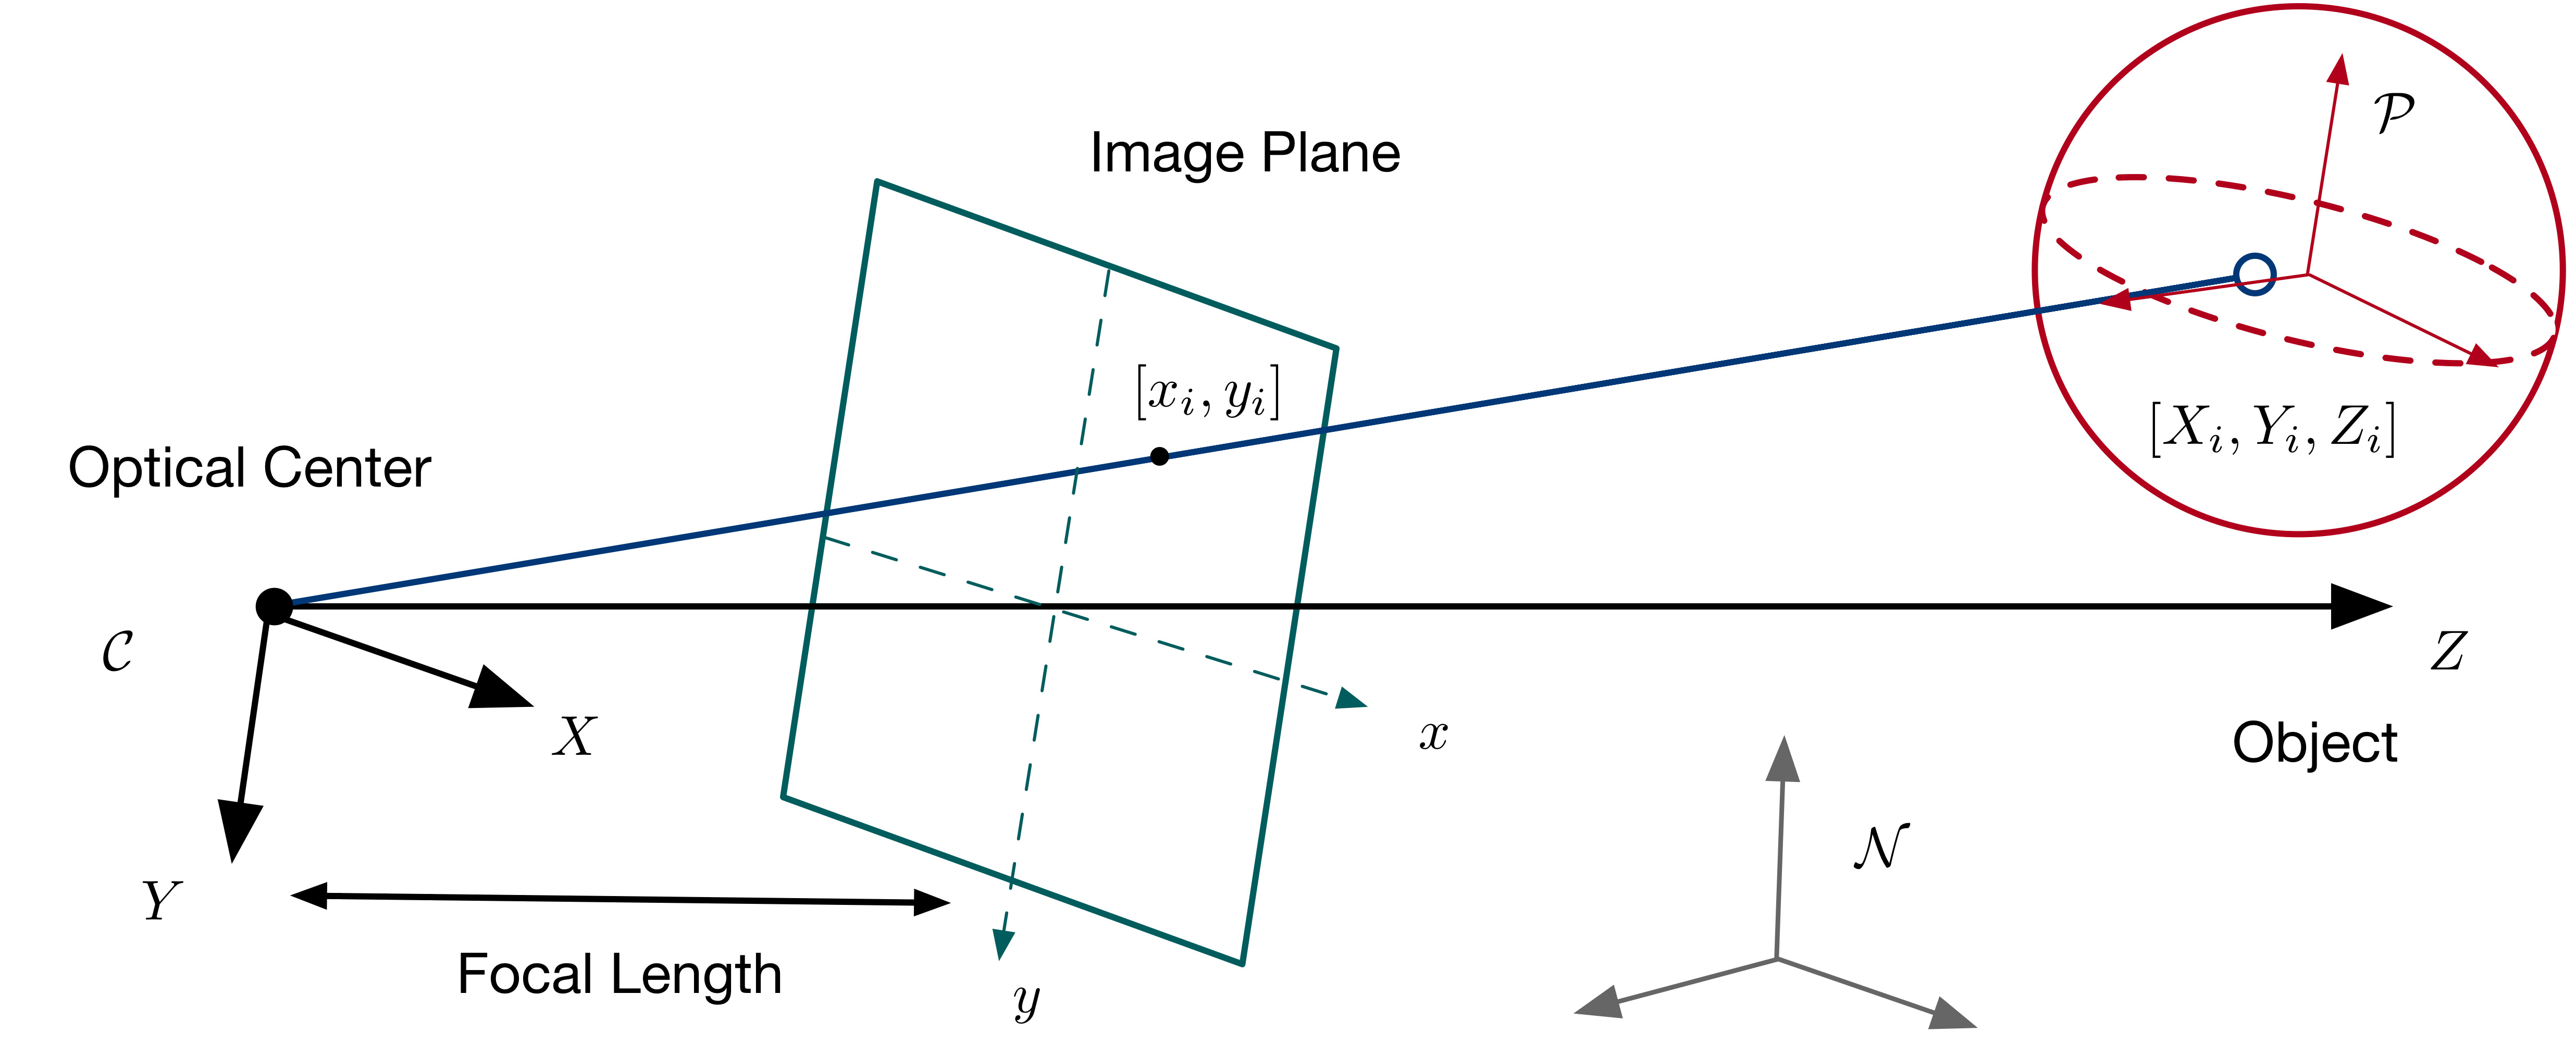
\includegraphics{Figures/CameraGeometry}
	}
	\caption{Camera Model}
	\label{fig:camera}
\end{figure}

\section{Model Description}

\subsection{Input and Output}

This converter module processes the output of a limb finding method to extract spacecraft inertial position. It does this by reading spacecraft attitude (coming from star tracker or other means), camera parameters, and the limb data. 

Messages read:

\begin{itemize}
\item CameraConfigMsg: containing focal length, resolution, and sensor size. These values are needed for the following computations. Notably the camera frame relative to the body frame is used.
\item LimbInMsg: Limb points, and uncertainty around these values in pixels. 
\item NavAttInMsg: Used for the spacecraft attitude. This allows to move from the body frame to the inertial frame.
\end{itemize}

Message written:
\begin{itemize}
\item OpNavFswMsg: Message containing $\leftexp{N}{\bm r}$ and it's covariance.
\end{itemize}

\subsection{Position computation}

The details of the algorithm are summarized in the papers attached. The engineering note contains a summary of the algorithms and covariance analysis. The journal paper \cite{Chirstian_Limb} contains the details of the development and assumptions. 

The component that is chosen in the implementation is the way to solve the least squares for equation $$[H] \bm x = \bm 1$$

This is done in this module by performing a QR-decomposition via a a Gram-Schmidt process. This leads to the following equation:

$$[R] \bm x = [Q]^T\bm 1$$

Since $[R]$ is upper-triangular, this is solved with an implemented back-substitution.  %This section includes mathematical models, code description, etc.

% !TEX root = ./Basilisk-MODULENAME-yyyymmdd.tex


\section{Module Functions}
This module 
\begin{itemize}
	\item \textbf{Compute atmospheric density and temperature}: Each of the provided models is fundamentally intended to compute the neutral atmospheric density and temperature for a spacecraft relative to a body. These parameters are stored in the AtmoPropsSimMsg struct. Supporting parameters needed by each model, such as planet-relative position, are also computed.
	\item \textbf{Communicate neutral density and temperature}: This module interfaces with modules that subscribe to neutral density messages via the messaging system.
	\item \textbf {Subscribe to model-relevant information:} Each provided atmospheric model requires different input information to operate, such as current space weather conditions and spacecraft positions. This module automatically attempts to subscribe to the relevant messages for a specified model. 
	\item \textbf{Support for multiple spacecraft and model types} Only one Atmosphere module is required for each planet, and can support an arbitrary number of spacecraft. Output messages for individual spacecraft are automatically named based on the environment type.
\end{itemize}

\section{Module Assumptions and Limitations}
Individual atmospheric models are complex and have their own assumptions. At present, all non-exponential models are Earth-specific. For details about tradeoffs in atmospheric modeling, the reader is pointed to ~\citenum{vallado2013}.  %This includes a concise list of what the module does. It also includes model assumptions and limitations

% !TEX root = ./Basilisk-thrFiringRemainder-2019-03-28.tex

\section{Test Description and Success Criteria}
The unit test creates a desired thruster force input vector and then runs the simulation for 3 seconds.  If the {\tt resetCheck} flag is true then a {\tt reset()} method is called and the simulation is repeated for another 2.5 seconds.  If the {\tt dvOn} flag is set than the off-pulsing mode is checked.  




\section{Test Parameters}

The simulation sets up 8 thrusters.  All permutations with the {\tt resetCheck} and {\tt dvOn} states are run.  The output is checked to the tolerance shown in Table~\ref{tab:errortol}.

\begin{table}[htbp]
	\caption{Error tolerance for each test.}
	\label{tab:errortol}
	\centering \fontsize{10}{10}\selectfont
	\begin{tabular}{ c | c } % Column formatting, 
		\hline\hline
		\textbf{Output Value Tested}  & \textbf{Tolerated Error}  \\ 
		\hline
		{\tt OnTimeRequest}        & 1e-05	   \\ 
		\hline\hline
	\end{tabular}
\end{table}




\section{Test Results}
All of the tests passed:
\begin{table}[H]
	\caption{Test results}
	\label{tab:results}
	\centering \fontsize{10}{10}\selectfont
	\begin{tabular}{c | c  | c } % Column formatting, 
		\hline\hline
		{\tt resetCheck} & {\tt dvOn} &\textbf{Pass/Fail} \\ 
		\hline
	   False & False	   			& \input{AutoTeX/passFailFalseFalse} \\ 
	   False & True	   			& \input{AutoTeX/passFailFalseTrue} \\ 
	   True & False	   			& \input{AutoTeX/passFailTrueFalse} \\ 
	   True & True	   			& \input{AutoTeX/passFailTrueTrue} \\ 
	   \hline\hline
	\end{tabular}
\end{table}



 % This includes test description, test parameters, and test results

\section{User Guide}

The model can be configured according to the user's wishes, but the following
rules of thumb should probably be respected unless the user is confident:
\begin{enumerate}
\item{The internal simulation dynamics step time should be less than or equal
     to the thruster ramp-up/ramp-down time steps}
\item{The internal simulation dynamics step time should be less than or equal to
     the desired thruster discretization level}
\item{The internal simulation dynamics step time should be less than one-tenth
    of the expected minimum allowable thruster firing duration}
\end{enumerate}

A common set up for thrusters, contains:

\begin{itemize}
  \item[-]      \texttt{thrusterSet = thrusterDynamicEffector.ThrusterDynamicEffector()}: Construct the Thruster Dyn Effector
  \item[-]   \texttt{thrusterSet.ModelTag = "ACSThrusterDynamics"}: Set the model tag
  \item[-]   \texttt{thruster1 = thrusterDynamicEffector.THRSimConfigMsgPayload()}: Create a individual thruster
  \item[-]   \texttt{thruster1.thrLoc\_B = [[1.0] ,[ 0.], [0.]] }: Set the thruster's location
  \item[-]   \texttt{thruster1.thrDir\_B = [[math.cos(anglerad)], [math.sin(anglerad)], [0.0]]}: Set the thruster thrust direction
  \item[-]   \texttt{thruster1.MaxThrust = 1.0}: Set the max thrust
  \item[-]   \texttt{thruster1.MaxSwirlTorque = 0.5}: Set the maximum swirl torque
  \item[-]   \texttt{thruster1.steadyIsp = 226.7}: Set the $I_{sp}$
  \item[-]   \texttt{thruster1.MinOnTime = 0.006}: Set the minimum on time
  \item[-]   \texttt{thrusterSet.addThruster(thruster1)}: Add thruster to the Dyn Effector
\end{itemize}

If attaching the thruster to a body, the last line is instead:

\begin{itemize}
     \item[-]   \texttt{thrusterSet.addThruster(thruster1, bodyStatesMsg)}: Add thruster to the Dyn Effector and attach it to a different body through the states message
\end{itemize}

If setting up a ramp, the user must also perform this:

\begin{itemize}
 \item[-]      \texttt{rampOnList = []}
 \item[-]      \texttt{rampOffList = []}

 \item[-]      \texttt{for i in range(rampsteps):}

\hspace{2cm}\texttt{fnewElement = thrusterDynamicEffector.THRTimePairSimMsg()}

\hspace{2cm}\texttt{fnewElement.TimeDelta = (i + 1.) * 0.1}

\hspace{2cm}\texttt{fnewElement.ThrustFactor = (i + 1.0) / 10.0}

\hspace{2cm}\texttt{fnewElement.IspFactor = (i + 1.0) / 10.0}

\hspace{2cm}\texttt{frampOnList.append(newElement)}

\hspace{2cm}\texttt{fnewElement = thrusterDynamicEffector.THRTimePairSimMsg()}

\hspace{2cm}\texttt{fnewElement.TimeDelta = (i + 1) * 0.1}

\hspace{2cm}\texttt{fnewElement.ThrustFactor = 1.0 - (i + 1.0) / 10.0}

 \hspace{2cm}\texttt{fnewElement.IspFactor = newElement.ThrustFactor}

 \hspace{2cm}\texttt{frampOffList.append(newElement)}

 \item[-]      \texttt{thrusterSet.thrusterData[0].ThrusterOnRamp =}

  \texttt{thrusterDynamicEffector.ThrusterTimeVector(rampOnList)}: Add the on ramp
 \item[-]      \texttt{thrusterSet.thrusterData[0].ThrusterOffRamp =}

 \texttt{thrusterDynamicEffector.ThrusterTimeVector(rampOffList)}: Add the off ramp
\end{itemize}

If setting up blow down effects, the user must also add these optional parameters to the thruster model before adding it to the set:

\begin{itemize}
  \item[-]   \texttt{thruster1.thrBlowDownCoeff = [1.0 , 2.0, 3.0] }: Set any number of polynomial coefficients for mass to thrust equation
  \item[-]   \texttt{thruster1.thrLoc\_B = [1.0 , 2.0, 3.0] }: Set any number of polynomial coefficients for mass to $I_{sp}$ equation
\end{itemize}
 % Contains a discussion of how to setup and configure  the BSK module






\bibliography{bibliography} %This includes references used and mentioned.

\end{document}
